%!TEX root = main.tex

\section{Resonance}

\begin{frame}
\frametitle{$\pi^{+}\pi^{-}$-system study at ALICE}
\begin{itemize}
	\item{$\pi^{+}\pi^{-}$-system study at ALICE}
\end{itemize}
\begin{table}[htp]
\begin{center}
\begin{tabular}{|c|c|}
\hline
Resonance  & paper\\
\hline
$K^0_{S} \rightarrow \pi^{+}\pi^{-}$ & Main topic of Strangeness group\\
$\rho^0(770) \rightarrow \pi^{+}\pi^{-}$ & Paper approval process \footnotemark\\
$f_0(980) \rightarrow \pi^{+}\pi^{-}$ & not yet \\
$f_2(1270) \rightarrow \pi^{+}\pi^{-}$ & not yet \\
\hline
\end{tabular}
\end{center}
\label{default}
\end{table}%

\begin{itemize}
	\item{$f_0(980) \rightarrow \pi^{+}\pi^{-}$, $f_2(1270) \rightarrow \pi^{+}\pi^{-}$}
	\begin{itemize}
		\item{More short-lived resonances than $\rho^0(770)$ ( $ c\tau$  $<$ 1.3 fm)}
		\item{To see also centrality dependent suppression of $f_0(980)$, $f_2(1270)$ as  $\rho^0(770)$ due to the rescattering of the daughter particles in the hadron gas.}
	\end{itemize}

\end{itemize}

\footnotetext{https://aliceinfo.cern.ch/ArtSubmission/node/3181}
\end{frame}

\begin{frame}
\frametitle{Data sample, event and track selection}
\begin{itemize}
\item{Event selection}
	\begin{itemize}
	\item{Trigger selection : Minimum-bias}
	\item{Vertex cut : $|z_\mathrm{vtx}|<10$ cm}
	\item{Centrality estimator : V0A\footnotemark[1] for p-Pb, V0M\footnotemark[2] for Pb-Pb}
	\end{itemize}
\item{Track selection}
	\begin{itemize}
	\item{Hybrid tracks (ITSTPC tracks + complementary tracks)\\ for primary track selection}
	\item{$p_\mathrm{T}^\mathrm{track}$ $>$ 0.15 GeV/$c$, $|\eta^\mathrm{track}|<0.9$}
	\item{PID : ALICE official Bayesian PID method applied  }
	\item{$|y_\mathrm{\pi^{+}\pi^{+}}|<0.5$}
	\end{itemize}
\item{Data sample}
\end{itemize}

\begin{table}[htp]
\begin{center}
\begin{tabular}{|c|c|}
\hline
Collision & Minimum bias and $|z_\mathrm{vtx}|<10$ cm \\ 
\hline
pp (LHC10b,c,d and e) & 240 millions \\
p-Pb (LHC13b and c) & 29 millions\\
Pb-Pb (LHC10h) & 15 millions\\
\hline

\end{tabular}
\end{center}
\label{default}
\end{table}%
\footnotetext[1]{VZERO-A side multiplicity}
\footnotetext[2]{The sum of VZERO-A and VZERO-C side multiplicities}
\end{frame}

\begin{frame}
\frametitle{Signal extraction}
\begin{columns}[c]
\column{.5\textwidth}
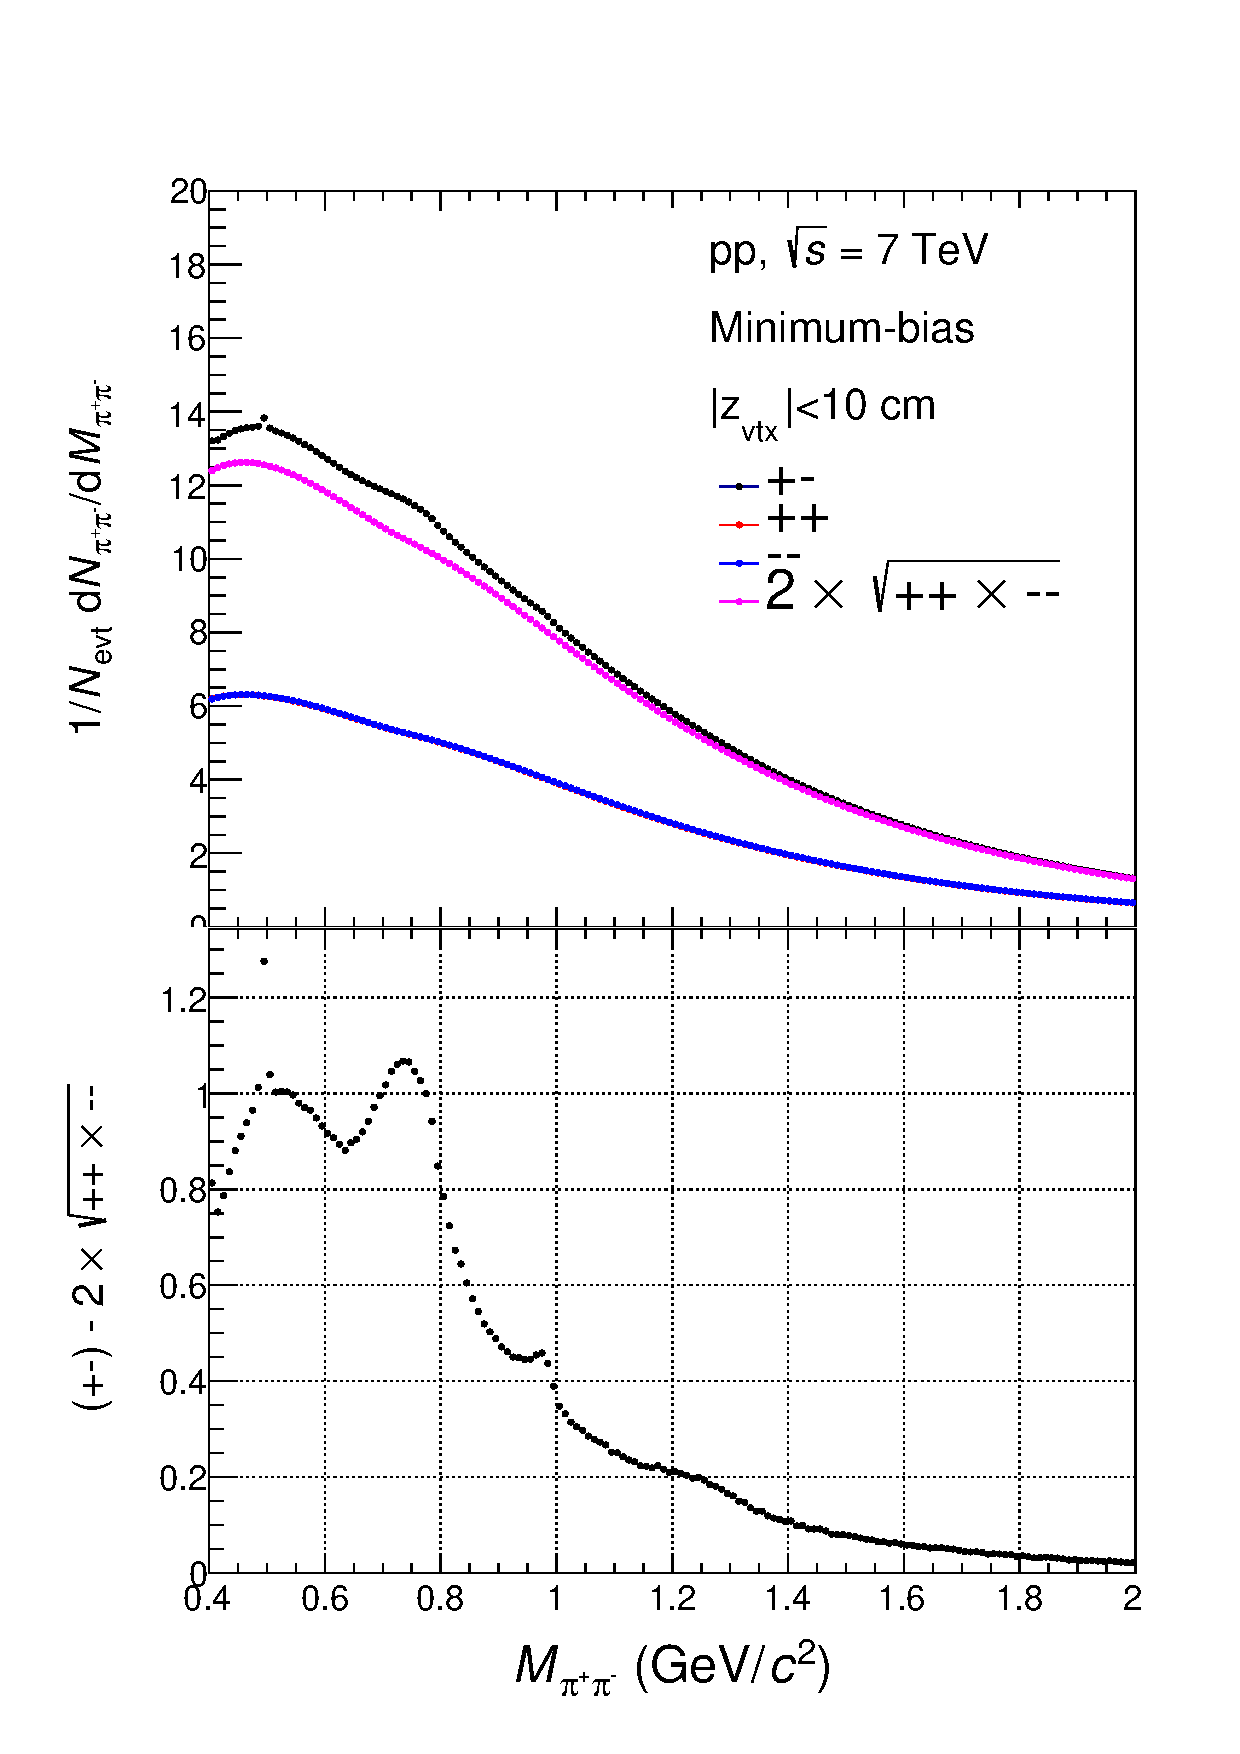
\includegraphics[width=1.\linewidth]{TwoPiondNdM}\\
\column{.5\textwidth}
Signal extraction
\begin{itemize}
\item{Unlike sign\\All combinations of \\ $\pi^{+}$ and $\pi^{-}$ in an event }
\item{like signs\\All combinations of\\ ($\pi^{+}$ and $\pi^{+}$)  or ($\pi^{-}$ and $\pi^{-}$) }
\item{Signal = unlike yield - geometric mean of two-like-sign yields}
\item{Study ongoing with the event-mixing method }

\end{itemize}
\end{columns}

\end{frame}

\begin{frame}
\frametitle{$f_0(980) \rightarrow \pi^{+}\pi^{-}$, $f_2(1270) \rightarrow \pi^{+}\pi^{-}$}
\begin{columns}[c]
\column{.5\textwidth}
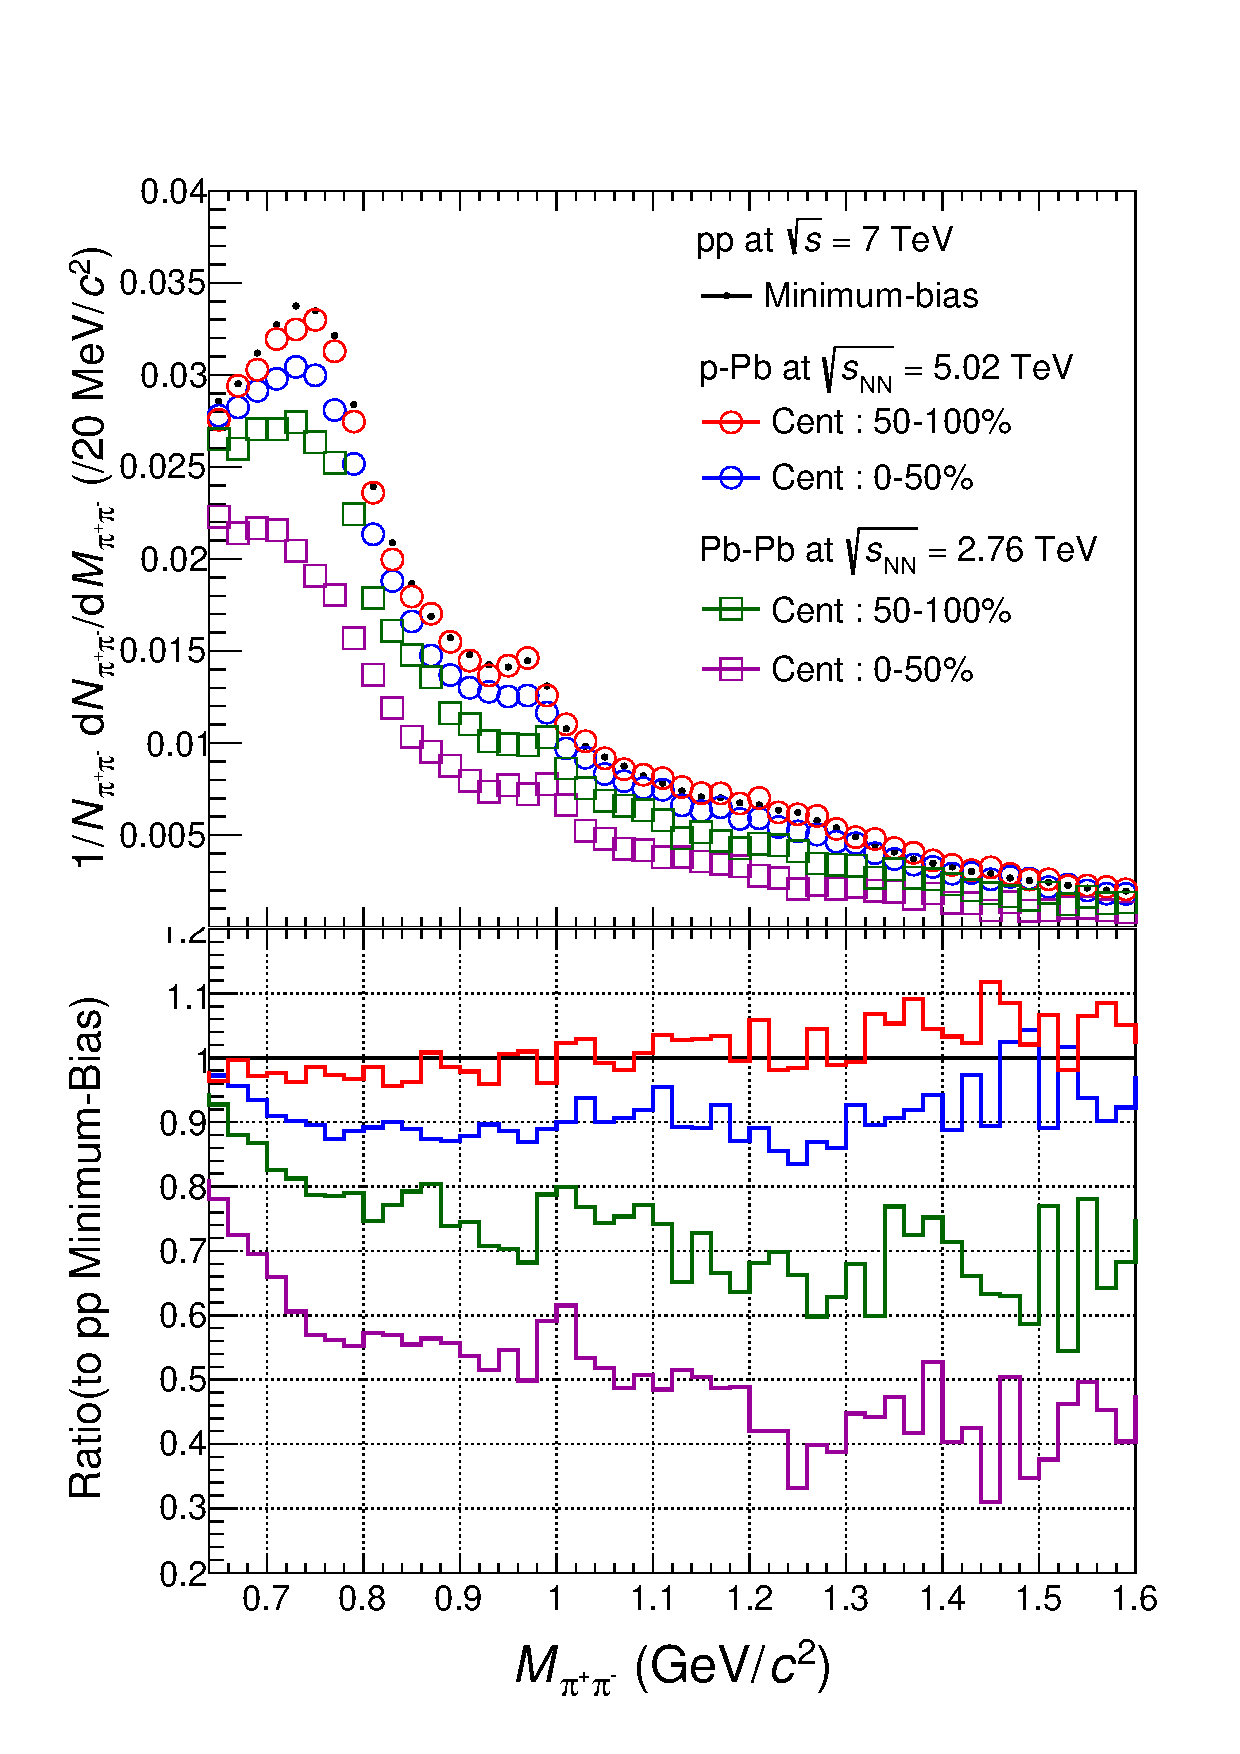
\includegraphics[width=1\linewidth]{../Figures/f0f2}\\
\column{.5\textwidth}
Inclusive $M_{\pi^{+}\pi^{-}}$  
\begin{itemize}
	\item{$f_2(1270)$ not clearly seen in central Pb-Pb events}
	\item{$f_0(980)$ shifts to higher mass in denser medium, but $\rho^0(770)$ behaves reversely   }
\end{itemize}
Study of yields w.r.t $p_\mathrm{T}^{\pi^{+}\pi^{-}}$ 
\begin{itemize}
\item{Essential for this study}
\item{Ongoing}
\end{itemize}

\end{columns}
\end{frame}





















